\let\negmedspace\undefined
\let\negthickspace\undefined
\documentclass[journal]{IEEEtran}
\usepackage[a5paper, margin=10mm, onecolumn]{geometry}
%\usepackage{lmodern} % Ensure lmodern is loaded for pdflatex
\usepackage{tfrupee} % Include tfrupee package

\setlength{\headheight}{1cm} % Set the height of the header box
\setlength{\headsep}{0mm}     % Set the distance between the header box and the top of the text

\usepackage{gvv-book}
\usepackage{gvv}
\usepackage{cite}
\usepackage{amsmath,amssymb,amsfonts,amsthm}
\usepackage{algorithmic}
\usepackage{graphicx}
\usepackage{textcomp}
\usepackage{xcolor}
\usepackage{txfonts}
\usepackage{listings}
\usepackage{enumitem}
\usepackage{mathtools}
\usepackage{gensymb}
\usepackage{comment}
%\usepackage{multiclo}
\usepackage[breaklinks=true]{hyperref}
\usepackage{tkz-euclide} 
\usepackage{listings}
\usepackage{tikz}
% \usepackage{gvv} 
\graphicspath{ {./figs/} }

\begin{document}
\title{ASSIGNMENT 2: GATE 2011 \\
MN: MINING ENGINEERING}
\author{AI25BTECH11010 - Dhanush Kumar A}
\maketitle
 \renewcommand{\thefigure}{\theenumi}
 \renewcommand{\thetable}{\theenumi}
\begin{enumerate}

\item A scatter plot prepared using a set of values of lead and zinc from a lead-zinc deposit is shown in figure below. The value of correlation coefficient is

\begin{center}
\includegraphics[width=0.4\textwidth]{Screenshot_2025_0813_154158.png} 
\end{center}

\begin{enumerate}
 \begin{multicols}{4}
    \item 1.0
    \item 0.7
    \item 0.5
    \item 0
    \end{multicols}
\end{enumerate}

\item The two vectors are orthonormal, if
\begin{enumerate}

    \item vector product is zero and norm of each vector is also zero
    \item vector product is one and norm of each vector is also one
    \item cross product is zero and norm of each vector is one
    \item cross product is one and norm of each vector is zero
    
\end{enumerate}

\item The value of 
\[
\lim_{x \to 0} \frac{1}{x} \left( \sqrt{1+x} - \sqrt{1-x} \right) \ \text{is}
\]
\begin{enumerate}
\begin{multicols}{4}
    \item 0
    \item 1
    \item 2
    \item 3
    \end{multicols}
\end{enumerate}

\item The infinite series $1 + \frac{1}{2} + \frac{1}{4} + \frac{1}{8} + \cdots$ is
\begin{enumerate}
\begin{multicols}{4}
    \item convergent
    \item divergent
    \item oscillatory
    \item semi-convergent
    \end{multicols}
\end{enumerate}

\item The largest area of a rectangular shaft for a given constant perimeter is obtained when length is
\begin{enumerate}
\begin{multicols}{2}
    \item 2.5 times of breadth
    \item 1.5 times of breadth
    \item 2 times of breadth
    \item equal to breadth
    \end{multicols}
\end{enumerate}

\item A drive shaft of an engine develops torque of $500$ N$\cdot$m. It rotates at a constant speed of $50$ rpm. The power transmitted by the shaft in kW is
\begin{enumerate}
\begin{multicols}{4}
    \item 1.46
    \item 2.05
    \item 2.62
    \item 4.32
    \end{multicols}
\end{enumerate}

\item A mine winder cage traveling $450$ m from pit bottom to pit top is following a three period duty cycle as shown in the figure below. The maximum velocity attained by the cage in m/s is

\begin{center}
\includegraphics[width=0.5\textwidth]{Screenshot_2025_0813_160511.png} 
\end{center}

\begin{enumerate}
		\begin{multicols}{4}
    \item 7.5
    \item 9.0
    \item 11.0
    \item 12.0
	    \end{multicols}
\end{enumerate}

\item Stress concentration at a point on the wall of a vertical shaft results in a compressive stress of $59.66$ MPa. The wall rock mass has an unconfined compressive strength of $89.49$ MPa. The safety factor of the shaft wall at the point is
\begin{enumerate}
\begin{multicols}{4}
    \item 0.67
    \item 0.86
    \item 1.23
    \item 1.50
	    \end{multicols}
\end{enumerate}

\item A core sample of $54$ mm diameter having Young$’$s modulus of $68.97$ GPa fails in uniaxial compression at $0.1\%$ axial strain. The axial load at failure in kN is
\begin{enumerate}
		\begin{multicols}{4}
    \item 158.00
    \item 68.97
    \item 58.00
    \item 15.80
	    \end{multicols}
\end{enumerate}

\item The maximum number of coal faces in an underground bord and pillar development district is 13. The number of headings in the district is
\begin{enumerate}
		\begin{multicols}{4}
    \item 3
    \item 5
    \item 6
    \item 7
	    \end{multicols}
\end{enumerate}

\item The whole circle bearing of the line AB is $116^\circ 20'20''$. If there exists an east declination of $20'$, the true quadrantal bearing of line AB is
\begin{enumerate}
\begin{multicols}{4}
    \item S$41^\circ 59'40''$E
    \item S$43^\circ 39'40''$E
    \item S$45^\circ 59'40''$W
    \item S$47^\circ 59'40''$W
	    \end{multicols}
\end{enumerate}

\item It is proposed to connect two straights of a road by a simple circular curve. If the maximum speed of the vehicle is 60 km/h and the centrifugal ratio for the road is 1/4, the minimum radius of the curve in m is
\begin{enumerate}
		\begin{multicols}{4}
    \item 113.26
    \item 98.18
    \item 25.46
    \item 15.50
	    \end{multicols}
\end{enumerate}

\item A centrifugal fan rotating at 500 rpm delivers $70$ m$^3$/s of air. If the speed is reduced to 200 rpm, the quantity of air delivered in m$^3$/s will be
\begin{enumerate}
		\begin{multicols}{4}
    \item 175
    \item 55
    \item 28
    \item 11
	    \end{multicols}
\end{enumerate}

\item According to mine regulations, the value of the fleet angle $\alpha$, in degree of a drum winder installation lies in the range of
\begin{enumerate}
		\begin{multicols}{4}
    \item $1.5 < \alpha \leq 2.0$
    \item $0 < \alpha \leq 1.5$
    \item $2.0 < \alpha \leq 2.5$
    \item $2.5 < \alpha \leq 3.0$
	    \end{multicols}
\end{enumerate}

\item Water will not be delivered by a centrifugal pump due to
\begin{enumerate}
		\begin{multicols}{2}
    \item lack of priming
    \item too low discharge head
    \item wrong direction of rotation
    \item partial obstruction at discharge outlet
	    \end{multicols}
\end{enumerate}

\item Match the following

\medskip
\begin{tabular}{ll}
	\textbf{Mine car type} & \textbf{Mode of unloading} \\
P. Granby & 1. Bottom opening \\
Q. Gable bottom & 2. Both side tilting \\
R. Drop bottom & 3. Single side opening \\
S. Rocker dump & 4. Both side opening
\end{tabular}

\medskip
\begin{enumerate}
		\begin{multicols}{2}
    \item P-2, Q-4, R-3, S-1
    \item P-4, Q-1, R-3, S-2
    \item P-3, Q-1, R-4, S-2
    \item P-3, Q-4, R-1, S-2
	    \end{multicols}
\end{enumerate}

\item Mean air temperature of a 450 m deep downcast shaft is $29^\circ$C and that of the upcast shaft is $37^\circ$C. The height of the motive column in m is
\begin{enumerate}
\begin{multicols}{4}
    \item 8.2
    \item 9.5
    \item 11.6
    \item 12.8
	    \end{multicols}
\end{enumerate}

\item The total pressure and the static pressure measured at a point in a ventilation duct are 20 mm and 10 mm of water gauge respectively. If density of air is $1.2\ \text{kg/m}^3$, the velocity of the air in m/s is
\begin{enumerate}
		\begin{multicols}{4}
    \item 14.08
    \item 12.78
    \item 8.53
    \item 6.24
	    \end{multicols}
\end{enumerate}

\item The type of fire extinguisher that must \textbf{NOT} be used in case of fire in an electric substation located in an underground metal mine is
\begin{enumerate}
		\begin{multicols}{4}
    \item multi-purpose dry chemical extinguisher
    \item CO$_2$ snow extinguisher
    \item dry chemical powder extinguisher
    \item foam extinguisher
	    \end{multicols}
\end{enumerate}

\item ISO 9000 Quality Systems \textbf{DO NOT} contain
\begin{enumerate}
		\begin{multicols}{4}
    \item legal provisions
    \item measurement
    \item document control
    \item standardization
	    \end{multicols}
\end{enumerate}

\item Air samples collected from the intake and the return gates of a retreating longwall face show methane concentration values of 0.1\% and 0.8\% respectively. The production from the longwall face is 2000 tonne/day and the air quantity circulating the face is 15 m$^3$/s. The rate of methane emission in m$^3$ per tonne of coal produced is
\begin{enumerate}
		\begin{multicols}{4}
    \item 11.0
    \item 9.5
    \item 5.5
    \item 4.5
	    \end{multicols}
\end{enumerate}

\item The time study data of an equipment deployed in a mine during a calendar month is given below.\\
Total working hours = 400\\
Total maintenance hours = 100\\
Total hours of actual work = 240\\
The percentage of utilization of the equipment is
\begin{enumerate}
		\begin{multicols}{4}
    \item 85
    \item 80
    \item 65
    \item 60
	    \end{multicols}
\end{enumerate}

\item 
100 ml of waste water is allowed to evaporate in a dish weighing 48.6232 g. The weight of the dish with dry solids is 48.6432 g. The concentration of dry solids in waste water in mg/l is 
\begin{enumerate}
		\begin{multicols}{4}
    \item 200
    \item 220
    \item 260
    \item 320
	    \end{multicols}
\end{enumerate}

\item 
A longwall face cut by double back shuffle method can be only worked with 
\begin{enumerate}
		\begin{multicols}{2}
    \item fixed drum shearer
    \item single ended ranging drum shearer
    \item double ended ranging drum shearer
    \item plough
	    \end{multicols}
\end{enumerate}

\item 
Proximate analysis of 50 g of a coal sample shows the following: \\
Moisture = 0.80 g \\
Ash = 7.85 g \\
Volatile matter = 15.90 g \\
The fixed carbon in percentage on a dry, ash free basis is 
\begin{enumerate}
		\begin{multicols}{4}
    \item 83
    \item 66
    \item 55
    \item 45
	    \end{multicols}
\end{enumerate}

\item 
For an oil exploration drilling, chance of striking an oil reservoir is 1 out of 15. If an oil exploration company decides to explore 5 sites, the probability of striking at least one successful oil reservoir is 
\begin{enumerate}
		\begin{multicols}{4}
    \item 0.292
    \item 0.250
    \item 0.034
    \item 0.0024
	    \end{multicols}
\end{enumerate}

\item 
Product of the eigen values of the matrix $A$ is 
\[
A = \begin{bmatrix}
3 & 2 & 5 \\
2 & 2 & 1 \\
1 & 5 & 4
\end{bmatrix}
\]
\begin{enumerate}
		\begin{multicols}{4}
    \item 6
    \item 8
    \item 10
    \item 35
	    \end{multicols}
\end{enumerate}

\item 
For the equation $\frac{dy}{dx} = 2x + 3y$, the value of $y$ at $x = 0.1$ in one step using Runge-Kutta fourth order method for the condition $y = 1$ when $x = 0$, is 
\begin{enumerate}
		\begin{multicols}{4}
    \item 0.3608
    \item 1.2508
    \item 1.3608
    \item 1.4625
	    \end{multicols}
\end{enumerate}

\item 
Value of the integral $\int_{0}^{1} \sqrt{\frac{1+x}{1-x}} \, dx$ is 
\begin{enumerate}
		\begin{multicols}{4}
    \item $\frac{\pi}{2} - 1$
    \item $\frac{\pi}{2} + 1$
    \item $\pi - 1$
    \item $\pi + 1$
	    \end{multicols}
\end{enumerate}

\item A 1 tonne mine car traveling at a constant speed o    f 10 km/h collides with a stationary buffer and co    mes to rest. If the buffer spring stiffness is 200     kN/m, the maximum compression in the spring in mm     is                        
\begin{enumerate}                                 
	\begin{multicols}{4}                     
	\item 49                                 
	\item 98                                 
	\item 196                                
	\item 247                                
	             \end{multicols}              
\end{enumerate}


\item In an iron ore handling port, a barge is pulled by ropes using two tugboats as shown in the figure. In equilibrium, the resultant of the forces $T_1$ and $T_2$ along the axis of the barge in the direction of its travel is $5000 \, \mathrm{N}$. The tensions $T_1$ and $T_2$ in N respectively are

\begin{center}
\includegraphics[width=0.4\textwidth]{Screenshot_2025_0813_192351.png}
\end{center}

\begin{enumerate}
		\begin{multicols}{2}
    \item 9700 and 6831
    \item 6831 and 9700
    \item 3660 and 2588
    \item 2588 and 3660
	    \end{multicols}
\end{enumerate}

\item A flat belt conveyor is carrying coal of bulk density $1\, \mathrm{tonne/m^3}$ at a rate of $400 \, \mathrm{tonne/h}$. The belt speed is $3\, \mathrm{m/s}$. Coal is spread over the belt covering 80\% of the belt width in a shape of a triangle. If the pile height is $1/4$ of the belt width, the width of the belt in mm is
\begin{enumerate}
		\begin{multicols}{4}
    \item 1109
    \item 909
    \item 709
    \item 609
	    \end{multicols}
\end{enumerate}

\item Match the following

\begin{tabular}{|>{\raggedright}m{5cm}|c|}

\textbf{Hydraulic system components} & \textbf{Symbols} \\

P Fixed displacement unidirectional flow pump & 1 \begin{tikzpicture}[scale=0.8,baseline=(current bounding box.center)]
        \draw (0,0) -- (0,0.5);
        \draw (0,0.5) -- (0.5,1) -- (0,1.5) -- (-0.5,1) -- cycle;
        \draw[dashed] (-0.5,1) -- (0.5,1);
        \draw (0,1.5) -- (0,2);
    \end{tikzpicture} \\
	

Q Fixed displacement unidirectional flow motor & 2\begin{tikzpicture}[scale=0.8,baseline=(current bounding box.center)]
        \draw (0,0) -- (0,0.4);
        \draw (0,0.4) circle (0.6);
        \fill (0,0.4) ++(0,0.25) -- (-0.25,-0.15) -- (0.25,-0.15) -- cycle;
        \draw (0,-0.2) -- (0,-0.6);
    \end{tikzpicture}
 \\
	
R Accumulator & 3 \begin{tikzpicture}[scale=0.8,baseline=(current bounding box.center)]
        \draw (-0.5,0) arc[start angle=180,end angle=360,radius=0.5];
        \draw (-0.5,0) -- (-0.5,1.2);
        \draw (0.5,0) -- (0.5,1.2);
        \draw (-0.5,1.2) arc[start angle=180,end angle=360,radius=0.5];
        \draw (0,-0.5) -- (0,0);
    \end{tikzpicture}\\
	
S Filter & 4 \begin{tikzpicture}[scale=0.8,baseline=(current bounding box.center)]
        \draw (0,0) -- (0,0.4);
        \draw (0,0.4) circle (0.6);
        \fill (0,0.4) ++(0,-0.25) -- (-0.25,0.15) -- (0.25,0.15) -- cycle;
        \draw (0,-0.2) -- (0,-0.6);
    \end{tikzpicture}

\end{tabular}

\begin{enumerate}
		\begin{multicols}{2}
    \item P-4, Q-2, R-3, S-1
    \item P-2, Q-4, R-3, S-1
    \item P-3, Q-2, R-1, S-4
    \item P-2, Q-3, R-1, S-4
\end{multicols}
\end{enumerate}

\item Match the following
\begin{tabular}{c c c}                
\textbf{Method of mining} & \textbf{Stope support} & \textbf{Ore loading}  \\   
P. Shrinkage stoping & 1. Insitu pillar & a. Overhead mucker  \\        
Q. Blasthole stoping & 2. Broken ore & b. Pneumatic autoloader \\              
R. Top slicing & 3. Timber mat & c. Load haul dumper  \\                
\end{tabular}

\begin{enumerate}
		\begin{multicols}{2}
    \item P-2-a, Q-1-c, R-3-b
    \item P-2-a, Q-3-c, R-1-b
    \item P-2-b, Q-3-c, R-1-a
    \item P-3-c, Q-2-a, R-1-b
	    \end{multicols}
\end{enumerate}

\item A typical case of gravity loading under complete lateral restraint in flat strata is shown in the figure below. The physico-mechanical parameters of the strata are given in the table. The in situ stresses $(\sigma_Z, \sigma_H)$ on the top of the coal seam in MPa are:

\begin{center}
\includegraphics[width=0.6\textwidth]{Screenshot_2025_0813_193403.png} 
\end{center}
\begin{table}[h!]
\centering
	\small{
\begin{tabular}{|c|c|c|c|c|}
\hline
\textbf{Strata} & \textbf{Thickness (m)} & \textbf{Specific Gravity} & \textbf{Young's  Modulus (GPa)} & \textbf{Shear Modulus (GPa)} \\
\hline
Sandstone & 50 & 2.35 & 26.40 & 12.50 \\
\hline
Shale & 25 & 2.15 & 20.50 & 8.25 \\
\hline
Coal & 20 & 1.52 & 2.41 & 0.95 \\
\hline

\end{tabular}
} 
\end{table}
\begin{enumerate}
\begin{multicols}{4}
    \item $(10.17, 2.54)$
    \item $(10.17, 3.69)$
    \item $(11.68, 3.69)$
    \item $(11.68, 2.54)$
	    \end{multicols}
\end{enumerate}



\end{enumerate}

\end{document}

